\documentclass[runningheads]{llncs}

\usepackage[T1]{fontenc}
\usepackage{graphicx}
\usepackage{amsmath}
\usepackage{amssymb}
\usepackage{booktabs}
\usepackage{multirow}
\usepackage{xcolor}
\usepackage{placeins}
\usepackage[hidelinks]{hyperref}
\renewcommand\UrlFont{\color{blue}\rmfamily}
\urlstyle{rm}

% Notation.
\newcommand{\LGE}{\mathrm{LGE}}
\newcommand{\Cz}{\mathrm{C0}}
\newcommand{\TT}{\mathrm{T2}}
\newcommand{\Img}{\mathbf{I}}
\newcommand{\sg}{\mathrm{sg}}
\newcommand{\warp}{\mathcal{W}}

\begin{document}

\title{MoSAIC: Motion- and Supervision-Aware Inference for\\
Myocardial Scar and Edema Segmentation from\\
Multi-Sequence and Cine CMR}
\titlerunning{MoSAIC}

\author{Anonymous Author(s)}
\authorrunning{Anonymous}
\institute{Institution masked for double-blind review}

\maketitle

\begin{abstract}
CMR pathology segmentation must account for variable sequences and
annotation sets. We present MoSAIC: Motion- and Super\-vision-Aware
Inference for Myocardial Scar and Edema Segmentation. The cascade uses
anatomy to condition multi-sequence and cine CMR decoding. Coarse cardiac anatomy supplies a spatial prior
for multi-sequence scar decoding, a dedicated edema-zone expert, and a cine
scar head using end-diastole (ED)-anchored motion and warped anatomy. Presence-gated encoding
and supervision-masked losses represent missing sequences and unannotated
classes. The edema expert predicts an injury zone for fusion of scar and edema.
On CARE-2026 CARE-Myo\-cardium official validation, the best MoSAIC Dice entries
are 0.6965 for MyoPS scar, 0.5983 for MyoPS edema and 0.2069 for CineMyoPS scar.
Compared with nnU-Net, these entries improve scar and cine scar Dice and raise
three-track mean Dice from 0.492 to 0.501. The retained internal five-fold table
requires recovery of its generation provenance; no module-causal or controlled
robustness conclusions are drawn.

\keywords{Myocardial pathology segmentation \and Multi-sequence CMR \and
Cine CMR \and Motion-derived evidence \and Partial supervision.}
\end{abstract}

% ===========================================================================
\section{Introduction}
% ===========================================================================

After acute myocardial infarction, scar marks irreversibly necrotic myocardium
while edema marks salvageable injured tissue. Their relation
guides reperfusion assessment~\cite{eitel2011cardiac,ibanez2015evolving}, and
CMR resolves them through complementary contrasts: LGE highlights
scar~\cite{kim1999relationship}, T2-weighted imaging highlights
edema~\cite{abdelaty2004delayed}, and bSSFP/C0 supplies anatomy. Automating
their joint delineation is the goal of the MyoPS benchmark
family~\cite{li2023myops,zhuang2019multivariate}.

The CARE-2026 setting emphasizes realistic heterogeneity in both image evidence
and annotation protocols. In multi-sequence CMR, training cases may contain LGE,
LGE+C0 or the full LGE+C0+T2 combination; 80 of 220 cases annotate edema, and
centers provide different anatomical label sets. Effective training therefore
requires the objective to respect the class set that each center annotated. In
cine-only CMR, scar is represented primarily through regional wall-motion
abnormality~\cite{zhang2019deeplearningcine,ding2025cinemyops}, making motion a
clinically meaningful signal for contrast-free pathology inference.

MoSAIC links coarse anatomy localization to three fine-stage experts
(Fig.~\ref{fig:pipeline}): multi-sequence scar/anatomy decoding, injury-zone
prediction ($\text{edema}\cup\text{scar}$), and cine scar prediction from
ED-anchored motion and warped anatomy. Its contributions are this cascade,
presence-gated input handling and supervision masking for heterogeneous labels,
and organizer-scored validation. These are architecture and evaluation
contributions, without claims of module-specific performance gains.

% ===========================================================================
\section{Related Work}
% ===========================================================================

MyoPS benchmarks joint scar and edema segmentation using three CMR
sequences~\cite{zhuang2019multivariate,li2023myops}. Related methods address flexible
sequence use~\cite{qiu2023myopsnet}, joint alignment and
segmentation~\cite{ding2023aligning}, and coarse-to-fine
localization~\cite{zhai2020coarsemyops,wang2022awsnet}. U-Net and nnU-Net provide
generic segmentation backbones~\cite{ronneberger2015unet,isensee2021nnunet}.
Methods for missing modalities represent variable inputs~\cite{havaei2016hemis,dorent2019hetero},
while partial-label losses account for unannotated
classes~\cite{shi2021marginal,zhou2019priorpartial,fidon2021labelsetloss}.
MoSAIC combines presence gating with per-class supervision masks.

Prior work on contrast-free inference uses cine
appearance~\cite{zhang2019deeplearningcine},
strain~\cite{scatteia2017strain,morales2021deepstrain}, or joint motion and
segmentation~\cite{qin2018jointmotion}. CineMyoPS combines anatomy with
motion~\cite{ding2025cinemyops}; MoSAIC likewise uses motion-derived evidence
for its cine scar head.

% ===========================================================================
\section{Preliminaries}
% ===========================================================================

\noindent\textbf{Problem setup.} A dataset is a set of tuples
$\mathcal{D}=\{(X_i, Y_i, \mathbf{m}_i, \mathbf{s}_i)\}$. The label map
$Y \in \{0,\dots,C\}^{D\times H\times W}$ uses the challenge classes
$\{$background, myocardium, LV, RV, edema, scar$\}$. For label fusion, we denote
the injury zone as $Z=\text{edema}\cup\text{scar}$ and recover pure edema after
scar prediction. Two acquisition regimes occur. In the
\emph{multi-sequence} regime $X=(\Img_\LGE,\Img_\Cz,\Img_\TT)$ and
$\mathbf{m}\in\{0,1\}^3$ records which sequences a center actually acquired,
with absent sequences zero-filled. In the \emph{cine} regime
$X=(I_0,\dots,I_{T-1})$ is a single bSSFP sequence sampled over the cardiac
cycle and anchored at end-diastole (ED). In both regimes
$\mathbf{s}\in\{0,1\}^{C}$ records which classes the originating center
annotated; $s_c=0$ means the label map is silent about class $c$, leaving its
underlying presence unspecified.

\noindent\textbf{Evaluation.} Internal cross-validation reports the Dice
similarity coefficient and the 95th-percentile Hausdorff distance (HD95, in mm)
computed in the resampled physical space. Organizer-scored validation uses the
CARE-Myocardium metrics, Dice and Hausdorff distance (HD, in mm).

% ===========================================================================
\section{Method}
% ===========================================================================

\begin{figure}[t]
\centering
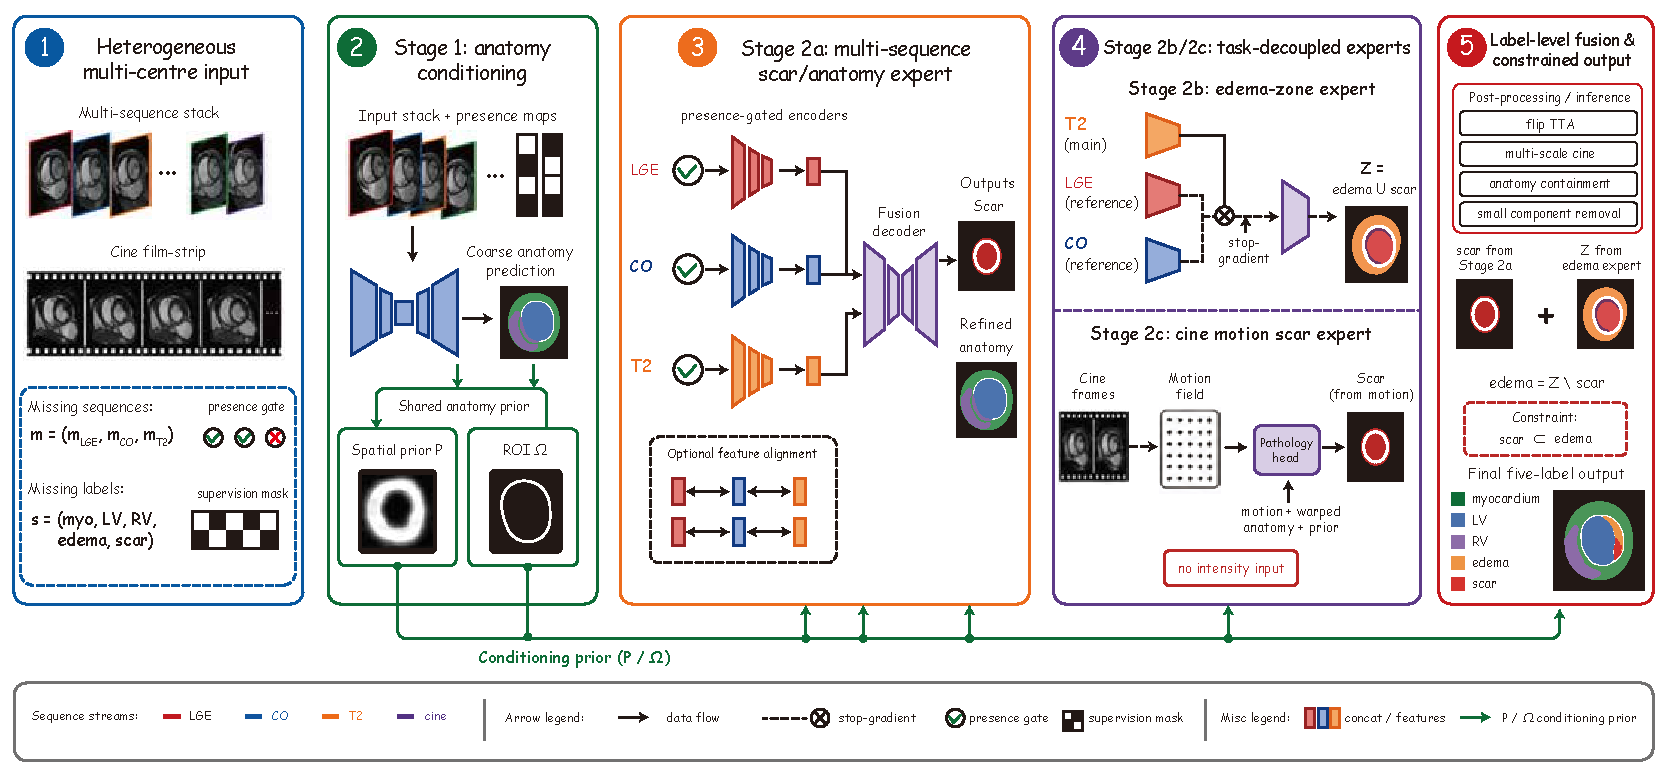
\includegraphics[width=\linewidth]{figures/fig1_original_redraw.pdf}
\caption{Overview of MoSAIC. A coarse anatomy stage defines the spatial prior;
separate multi-sequence scar, edema-zone, and cine-motion branches produce
task-specific predictions that are fused in the challenge label space. $Z$ denotes the injury
zone; final pure edema excludes scar.}
\label{fig:pipeline}
\end{figure}

Stage~1 supplies anatomy and a spatial prior to the multi-sequence scar,
edema-zone and cine-motion experts.

\subsection{Stage 1: Anatomy Conditioning}

A compact 2D U-Net~\cite{ronneberger2015unet} $F_{\text{coarse}}$ predicts three
coarse classes (myocardial ring, LV, RV) from the channel-stacked sequences
augmented with constant \emph{presence maps}, i.e.\ the input is
$[\Img_\LGE,\Img_\Cz,\Img_\TT, m_1\mathbf{1}, m_2\mathbf{1}, m_3\mathbf{1}]$.
Presence maps distinguish missing sequences from dark tissue. Thresholding and
largest-component selection give $\hat{Y}^{\mathrm{c}}$ and
$P=\mathbf{1}[\hat{Y}^{\mathrm{c}}>0]$. The dilated bounding box of $P$ defines
Stage~2's region of interest $\Omega$. Cine uses myocardium and LV coarse classes.

\subsection{Stage 2a: Multi-Sequence Scar and Anatomy Decoding}

Stage~2a predicts scar from LGE-centered features with auxiliary myocardium
decoding; Stage~2b handles edema.

\noindent\textbf{Modality-decoupled encoding with presence gating.} The framework
runs three independent encoders
$E^{(m)}$, $m\in\{\LGE,\Cz,\TT\}$, each producing a four-level pyramid
$f^{(m)}_\ell$, $\ell=1,\dots,4$. Missing sequences are suppressed
multiplicatively,
\begin{equation}
\tilde{f}^{(m)}_\ell \;=\; m_m \cdot f^{(m)}_\ell ,
\end{equation}
so an absent auxiliary sequence contributes no image-derived feature maps; the
decoder still receives fixed sigmoid gate values from the zeroed features. The
same weights serve LGE-only, LGE+C0 and full three-sequence cases.

\noindent\textbf{An optional alignment branch.} Separate breath-holds can
introduce fine non-rigid offsets around the thin myocardial ring where lesion
decisions are made. The framework therefore includes a deformable branch that models
sequence alignment inside the representation the decoder consumes: for each moving
sequence $m\in\{\Cz,\TT\}$ a localization head $h^{(m)}$ reads the \emph{paired}
bottlenecks and predicts $K=g^2$ control-point offsets
$\theta^{(m)}=h^{(m)}([\tilde{f}^{(m)}_4, f^{(\LGE)}_4])$, defining a thin-plate
spline~\cite{bookstein1989principal} $\mathcal{T}_{\theta}$ that warps every
pyramid level of that sequence (Appendix~\ref{app:tps}). The final head layer is initialized as described in Appendix~\ref{app:tps}.
TPS, prior gating and consistency are enabled in the final scar configuration.

\noindent\textbf{Fusion and prior gating.} The decoder fuses the sequence
pyramids with a gating rule that keeps LGE as the structural carrier while the
other sequences modulate it, and the Stage-1 prior re-enters at every decoder
level as a multiplicative gate that emphasizes the cardiac region while retaining
context. Appendix~\ref{app:fusion} gives the equations and the fixed gate
values induced by absent auxiliary sequences.

\subsection{A Supervision-Masked Objective for Ragged Annotation}

Training pools cases with different annotated class subsets by applying the
per-class supervision mask $\mathbf{s}$ directly in the loss normalizer. With $\ell^{\text{dice}}_{b,c}$ and
$\ell^{\text{bce}}_{b,c}$ the per-sample per-class Dice and binary
cross-entropy terms and $w_c$ a class weight,
\begin{equation}
\mathcal{L}_{\text{seg}}
=\frac{\sum_{b,c}\,s_{b,c}\,w_c\left[\ell^{\text{dice}}_{b,c}+\ell^{\text{bce}}_{b,c}\right]}
       {\sum_{b,c}\,s_{b,c}} .
\label{eq:masked}
\end{equation}
Each annotated class contributes its supervised gradient; an unannotated class
receives zero weight in both the numerator and the denominator. A case from a
scar-focused center therefore supervises the scar head and leaves edema
supervision to centers that annotated edema.

Small lesions additionally receive a recall-oriented Tversky
term~\cite{salehi2017tversky} with $\alpha<\beta$ and a focal
term~\cite{lin2017focal}, both restricted to lesion channels and both masked the
same way. Deep supervision is applied at two decoder levels.

An auxiliary \emph{cross-sequence myocardium consistency} term completes
Stage~2a (Appendix~\ref{app:losses}). It decodes a myocardium mask from each
sequence-specific feature stack and regularizes all available pairs with Dice
agreement. This ties representations through shared anatomy without adding
annotations.

\subsection{Stage 2b: A Dedicated Edema Expert}

The dedicated edema expert uses T2-driven evidence with scar and edema
supervision available on 220 and 80 cases, respectively.

The framework therefore trains a separate expert. T2 forms the main stream while the
LGE and C0 streams are fused element-wise into a \emph{reference} pyramid
$e^{\text{ref}}_\ell$, which enters the decoder \emph{detached},
$d_\ell=\Psi_\ell([\mathrm{up}(d_{\ell+1}),\,\sg(e^{\text{ref}}_\ell),\,e^{\TT}_\ell])$.
The detached reference supplies anatomical context without receiving gradients
through this decoder connection.

The expert regresses the injury zone $Z=\text{edema}\cup\text{scar}$, matching
the label representation used for fusion. Pure edema is recovered at fusion time
by assigning the predicted scar first and then filling
$Z\setminus\widehat{\text{scar}}$ as edema.

\subsection{Stage 2c: Motion-Derived Scar from Cine}

For cine-only data, the framework replaces the multi-sequence encoder stack with a
motion extractor. A shared encoder embeds each of $T$ ED-anchored frames; an
anatomy decoder predicts per-frame myocardium and LV; and a motion decoder
predicts a dense displacement field between the ED reference $I_0$ and frame
$I_t$, bounded to keep it physically plausible:
\begin{equation}
\varphi_t=\tau\tanh\!\left(D_{\text{mot}}(f_0,f_t)\right),\qquad \varphi_0=\mathbf{0},
\end{equation}
with $\tau$ the maximum displacement as a fraction of the field of view. The
field warps both the anatomy probability and the frame,
$\hat{A}_t=\warp(\sigma(A_t),\varphi_t)$ and $\hat{I}_t=\warp(I_t,\varphi_t)$.

The pathology head receives only motion, warped anatomy and the anatomical prior:
\begin{equation}
z_t=\Theta\!\left(\left[\varphi_t,\;\hat{A}_t,\;P\right]\right),
\qquad
\hat{Y}=\mathrm{Conv}_{1\times1}\!\left(\tfrac{1}{T}\textstyle\sum_{t} z_t\right).
\label{eq:cinehead}
\end{equation}
This restricts the cine scar branch to contrast-free temporal and anatomical
cues.

Training combines the masked pathology loss with four auxiliary terms: ED-frame
anatomy supervision; consistency between each warped anatomy map and the ED
prediction; a photometric term matching $\hat{I}_t$ to $I_0$; and an $\ell_1$
smoothness penalty on $\nabla\varphi$ for the displacement field.

\subsection{Inference}

Both regimes share one skeleton: predict anatomy, restrict to the prior, predict
pathology with flip test-time augmentation, then apply anatomical containment and
minimum lesion-size cleanup.
For the multi-sequence regime, scar comes from the Stage-2a scar/anatomy expert,
and edema is assigned from $Z\setminus\widehat{\text{scar}}$ under the injury-zone
fusion convention. For cine, predictions are additionally averaged over three
through-plane resamplings as the deployment-time handling of through-plane
resolution variation.

% ===========================================================================
\section{Experiments}
\label{sec:exp}
% ===========================================================================

\noindent\textbf{Data and data-use declaration.} All experiments use the
CARE-2026 CARE-Myocardium dataset, comprising the MyoPS multi-sequence cohort
and the CineMyoPS cine cohort. We use no other data. We gratefully acknowledge
the challenge organizers, and cite the sources as required:
\cite{zhuang2019multivariate,qiu2023myopsnet,ding2023aligning,ding2025cinemyops}.
Table~\ref{tab:cohort} summarises the heterogeneity that motivates our design.
No pre-trained weights are used; every model is trained from scratch.

\begin{table}[t]
\centering
\caption{The CARE-2026 CARE-Myocardium training cohort. Sequence availability and
annotated classes both vary by center: 116 of 220 multi-sequence cases provide LGE
alone, and 80 carry edema labels. The evaluation cohort provides all three
sequences, so a model can learn from partial training protocols and exploit
complete inputs at test time.}
\label{tab:cohort}
\setlength{\tabcolsep}{5pt}
\begin{tabular}{llll}
\toprule
Centre & Cases & Sequences & Annotated classes \\
\midrule
\multicolumn{4}{l}{\textit{MyoPS (multi-sequence)}}\\
A & 81 & LGE & myo, LV, scar \\
B & 35 & LGE+C0+T2 & myo, LV, RV, edema, scar \\
C & 45 & LGE+C0+T2 & myo, LV, RV, edema, scar \\
E & 7 & LGE+C0 & myo, LV, RV, scar \\
F & 9 & LGE+C0 & myo, LV, RV, scar \\
G & 8 & LGE+C0 & myo, LV, RV, scar \\
H & 35 & LGE & scar \\
\midrule
\multicolumn{4}{l}{\textit{CineMyoPS (cine only)}}\\
$\alpha$ & 40 & Cine & myo, LV, scar \\
$\beta$ & 24 & Cine & myo, LV, scar \\
\bottomrule
\end{tabular}
\end{table}

\noindent\textbf{Implementation.} Volumes are resampled to
$1.25\times1.25\times10.0$\,mm (multi-sequence) and
$1.25\times1.25\times8.0$\,mm (cine), robustly z-scored per volume, and processed
slice-wise at $192\times192$. Stage-1 uses 24 base channels, Stage-2a 24, the
edema expert 64 and the cine model 16, with instance
normalization~\cite{ulyanov2016instance}. We train with
AdamW~\cite{loshchilov2019adamw} under a cosine schedule~\cite{loshchilov2017sgdr},
gradient clipping at 0.1, and a class-quota batch sampler that guarantees a fixed
fraction of lesion-bearing slices per batch. The TPS warm-up is $E_w=10$ epochs.
The retained evaluation uses five folds; MyoPS has 176 training and 44
validation cases per fold, and CineMyoPS validation sizes are 13, 13, 13, 13 and 12. Because edema is
annotated at two centers, edema metrics are computed on those centers'
cases. Seed 3407 is a configuration default; the exact seeds and training
manifests for the final checkpoints remain unresolved.

\noindent\textbf{Metrics.} Internal five-fold results are reported as Dice
and HD95 (mm), with mean\,$\pm$\,standard deviation across folds. Official
validation results are organizer-reported Dice and HD (mm).

\subsection{Main Results}

\begin{table}[t]
\centering
\caption{Author-retained five-fold results, mean\,$\pm$\,s.d.\ across folds;
table-generation provenance remains unresolved. Pure-edema metrics use cases with edema annotations; the remaining
metrics use their corresponding annotated cohorts. Cine scar uses motion and anatomy, without contrast-enhanced input.}
\label{tab:main}
\begin{tabular}{lcc}
\toprule
Structure & Dice $\uparrow$ & HD95 (mm) $\downarrow$ \\
\midrule
\multicolumn{3}{l}{\textit{MyoPS: multi-sequence (LGE, C0, T2)}}\\
\quad Myocardium & 0.687\,{\tiny $\pm$\,0.036} & 8.29\,{\tiny $\pm$\,1.61} \\
\quad LV & 0.866\,{\tiny $\pm$\,0.015} & 5.87\,{\tiny $\pm$\,1.43} \\
\quad RV & 0.841\,{\tiny $\pm$\,0.022} & 6.63\,{\tiny $\pm$\,1.80} \\
\quad Pure edema & 0.349\,{\tiny $\pm$\,0.065} & 20.21\,{\tiny $\pm$\,3.49} \\
\quad Scar & 0.668\,{\tiny $\pm$\,0.022} & 11.69\,{\tiny $\pm$\,1.06} \\
\quad Lesion union & 0.645\,{\tiny $\pm$\,0.024} & 15.87\,{\tiny $\pm$\,3.13} \\
\midrule
\multicolumn{3}{l}{\textit{CineMyoPS: cine only}}\\
\quad Myocardium & 0.695\,{\tiny $\pm$\,0.024} & 5.35\,{\tiny $\pm$\,0.30} \\
\quad LV & 0.919\,{\tiny $\pm$\,0.007} & 3.87\,{\tiny $\pm$\,0.55} \\
\quad Scar & 0.457\,{\tiny $\pm$\,0.038} & 19.68\,{\tiny $\pm$\,3.88} \\
\bottomrule
\end{tabular}
\end{table}

\noindent\textbf{Official validation leaderboard.} Table~\ref{tab:leaderboard}
reports the best MoSAIC organizer-scored CARE-2026 validation entries for each
official target, using the organizer metrics Dice and HD. The best MoSAIC entries
reach $0.6965$ Dice for MyoPS scar, $0.5983$ for MyoPS edema and $0.2069$ for
CineMyoPS scar. Compared with the nnU-Net comparator, MoSAIC improves MyoPS scar,
CineMyoPS scar, and the mean Dice over the three official targets ($0.492$ to
$0.501$).


Table~\ref{tab:main} retains the author-approved attachment results without
additional performance claims. The source of the generated table remains unresolved. These local values
are distinct from official validation.

\begin{table}[t]
\centering
\caption{Best organizer-scored MoSAIC entries and the nnU-Net comparator on the
CARE-2026 validation leaderboards, reported as Dice/HD (mm). For each target, the
MoSAIC row is the submitted entry with the highest Dice.}
\label{tab:leaderboard}
\begin{tabular}{llcc}
\toprule
Leaderboard & Target & MoSAIC Dice/HD & nnU-Net Dice/HD \\
\midrule
MyoPS & scar & 0.6965 / 13.7827 & 0.6258 / 14.9844 \\
MyoPS & edema & 0.5983 / 26.7067 & 0.6691 / 21.0898 \\
CineMyoPS & scar & 0.2069 / 48.7463 & 0.1816 / 52.9706 \\
\bottomrule
\end{tabular}
\end{table}


\FloatBarrier
\subsection{Discussion}

MoSAIC combines anatomy conditioning, input-presence gates and case-aware
supervision. Its best official entries improve MyoPS and CineMyoPS scar Dice
relative to nnU-Net, with three-track mean Dice increasing from 0.492 to 0.501.
The per-track best-Dice entries do not establish mean HD improvement.

\noindent\textbf{Limitations.} The retained five-fold table lacks recovered
table-generation provenance. Full edema-stage folds 1--4 and local CineMyoPS
prediction/ground-truth evaluation artifacts remain unavailable in the evidence
package. Clean ablations and controlled sequence-withdrawal evaluation are also
missing; module-causal gains, controlled modality robustness, state-of-the-art
performance and cross-center robustness are not established. Cine folds are drawn from the same source centers,
whereas official validation may change scanner, frame count, temporal resolution
and slice thickness; protocol-normalized flow or explicit frame-rate augmentation
is therefore a natural extension. For edema, the current fusion predicts
$Z=\text{edema}\cup\text{scar}$ and obtains pure edema by subtracting scar at
fusion time. Further work will focus on strengthening edema supervision,
calibrating edema-zone fusion and adding inter-slice context.

% ===========================================================================
\section{Conclusion}
% ===========================================================================

MoSAIC uses coarse anatomy to condition pathology decoding, with input
presence gates, supervision masking, an edema-zone expert and cine motion
evidence. The best official validation Dice scores are
$0.6965$ for MyoPS scar, $0.5983$ for MyoPS edema and $0.2069$ for CineMyoPS
scar. These results support the reported validation endpoints without resolving
the limitations of the retained internal evaluation.

\bibliographystyle{splncs04}
\bibliography{refs}

% ===========================================================================
\appendix
% ===========================================================================

\section{Thin-Plate Spline Alignment Field}
\label{app:tps}

With target control points $\{p_k\}$ on a regular $g\times g$ lattice spanning
$[-r,r]^2$ and predicted offsets $\theta^{(m)}_k$, the thin-plate
spline~\cite{bookstein1989principal} is the interpolant of
$\{p_k\mapsto\theta^{(m)}_k\}$ with minimal bending energy:
\begin{equation}
\mathcal{T}_{\theta}(q) \;=\; a_0 + A\,q \;+\; \sum_{k=1}^{K} w_k\,U\!\left(\lVert q-p_k\rVert\right),
\qquad U(d)=d^2\log d ,
\end{equation}
where $(w,a_0,A)$ solve the standard TPS linear system. That system depends only
on $\{p_k\}$, which are fixed, so it is inverted once and cached. The final
linear layer of the localization head $h^{(m)}$ is zero-initialized with its bias
set to the target lattice, giving a stable starting warp that is updated by the
task loss.

\section{Cross-Modality Gated Fusion}
\label{app:fusion}

The Stage-2a decoder fuses the aligned pyramids at level $\ell$ as
\begin{align}
a_\ell &= \tfrac{1}{2}\left[\sigma\!\left(\hat{f}^{(\Cz)}_\ell\right) + \sigma\!\left(\hat{f}^{(\TT)}_\ell\right)\right],\\
d_\ell &= \Phi_\ell\!\left(\left[\,\mathrm{up}(d_{\ell+1}),\;\; f^{(\LGE)}_\ell\odot a_\ell,\;\; \sigma\!\left(\hat{f}^{(\Cz)}_\ell\right),\;\; \sigma\!\left(\hat{f}^{(\TT)}_\ell\right)\right]\right),
\end{align}
initialized from the concatenated bottlenecks
$d_4=[f^{(\LGE)}_4,\hat{f}^{(\Cz)}_4,\hat{f}^{(\TT)}_4]$. When an auxiliary
sequence is absent, its masked feature pyramid is zero, so its sigmoid gate
channel is fixed at $\sigma(0)=\tfrac12$. This is a consequence of the gate
parameterization, not an identity gate; the absent sequence contributes no
image-derived feature map. The Stage-1 prior gates every decoder level,
$d_\ell \leftarrow d_\ell\odot\sigma(\mathrm{pool}(P))$.

\section{Auxiliary Training Objectives}
\label{app:losses}

\noindent\textbf{Cross-sequence myocardium consistency.} Three auxiliary heads
$g^{(m)}$ decode a myocardium mask from each sequence's own features. For the
available sequences $A=\{m:m_m=1\}$, each head is supervised against the
myocardium label and every available pair in
$\mathcal{Q}=\{(m,m'):m<m',\,m,m'\in A\}$ is driven into agreement:
\begin{equation}
\mathcal{L}_{\text{cons}}=\frac{\mathcal{L}_{\text{sup}}+
\mathcal{L}_{\text{pair}}}{N},\qquad N=|A|+|\mathcal{Q}|.
\end{equation}
Here $\mathcal{L}_{\text{sup}}$ sums the sequence-specific myocardium Dice
terms, and $\mathcal{L}_{\text{pair}}$ sums the pairwise Dice agreement terms.

\noindent\textbf{Stage-2b edema expert.} The reference pyramid is formed as
\begin{equation}
e^{\text{ref}}_\ell=\max\!\left(E^{\LGE}_\ell([\Img_\LGE,M]),\;E^{\Cz}_\ell([\Img_\Cz,M])\right),
\qquad
e^{\TT}_\ell=E^{\TT}_\ell([\Img_\TT,M]),
\end{equation}
with $M$ a dilated cardiac mask from Stage~1.

\end{document}
